% Options for packages loaded elsewhere
% Options for packages loaded elsewhere
\PassOptionsToPackage{unicode}{hyperref}
\PassOptionsToPackage{hyphens}{url}
\PassOptionsToPackage{dvipsnames,svgnames,x11names}{xcolor}
%
\documentclass[
  letterpaper,
  DIV=11,
  numbers=noendperiod]{scrartcl}
\usepackage{xcolor}
\usepackage{amsmath,amssymb}
\setcounter{secnumdepth}{-\maxdimen} % remove section numbering
\usepackage{iftex}
\ifPDFTeX
  \usepackage[T1]{fontenc}
  \usepackage[utf8]{inputenc}
  \usepackage{textcomp} % provide euro and other symbols
\else % if luatex or xetex
  \usepackage{unicode-math} % this also loads fontspec
  \defaultfontfeatures{Scale=MatchLowercase}
  \defaultfontfeatures[\rmfamily]{Ligatures=TeX,Scale=1}
\fi
\usepackage{lmodern}
\ifPDFTeX\else
  % xetex/luatex font selection
\fi
% Use upquote if available, for straight quotes in verbatim environments
\IfFileExists{upquote.sty}{\usepackage{upquote}}{}
\IfFileExists{microtype.sty}{% use microtype if available
  \usepackage[]{microtype}
  \UseMicrotypeSet[protrusion]{basicmath} % disable protrusion for tt fonts
}{}
\makeatletter
\@ifundefined{KOMAClassName}{% if non-KOMA class
  \IfFileExists{parskip.sty}{%
    \usepackage{parskip}
  }{% else
    \setlength{\parindent}{0pt}
    \setlength{\parskip}{6pt plus 2pt minus 1pt}}
}{% if KOMA class
  \KOMAoptions{parskip=half}}
\makeatother
% Make \paragraph and \subparagraph free-standing
\makeatletter
\ifx\paragraph\undefined\else
  \let\oldparagraph\paragraph
  \renewcommand{\paragraph}{
    \@ifstar
      \xxxParagraphStar
      \xxxParagraphNoStar
  }
  \newcommand{\xxxParagraphStar}[1]{\oldparagraph*{#1}\mbox{}}
  \newcommand{\xxxParagraphNoStar}[1]{\oldparagraph{#1}\mbox{}}
\fi
\ifx\subparagraph\undefined\else
  \let\oldsubparagraph\subparagraph
  \renewcommand{\subparagraph}{
    \@ifstar
      \xxxSubParagraphStar
      \xxxSubParagraphNoStar
  }
  \newcommand{\xxxSubParagraphStar}[1]{\oldsubparagraph*{#1}\mbox{}}
  \newcommand{\xxxSubParagraphNoStar}[1]{\oldsubparagraph{#1}\mbox{}}
\fi
\makeatother


\usepackage{longtable,booktabs,array}
\usepackage{calc} % for calculating minipage widths
% Correct order of tables after \paragraph or \subparagraph
\usepackage{etoolbox}
\makeatletter
\patchcmd\longtable{\par}{\if@noskipsec\mbox{}\fi\par}{}{}
\makeatother
% Allow footnotes in longtable head/foot
\IfFileExists{footnotehyper.sty}{\usepackage{footnotehyper}}{\usepackage{footnote}}
\makesavenoteenv{longtable}
\usepackage{graphicx}
\makeatletter
\newsavebox\pandoc@box
\newcommand*\pandocbounded[1]{% scales image to fit in text height/width
  \sbox\pandoc@box{#1}%
  \Gscale@div\@tempa{\textheight}{\dimexpr\ht\pandoc@box+\dp\pandoc@box\relax}%
  \Gscale@div\@tempb{\linewidth}{\wd\pandoc@box}%
  \ifdim\@tempb\p@<\@tempa\p@\let\@tempa\@tempb\fi% select the smaller of both
  \ifdim\@tempa\p@<\p@\scalebox{\@tempa}{\usebox\pandoc@box}%
  \else\usebox{\pandoc@box}%
  \fi%
}
% Set default figure placement to htbp
\def\fps@figure{htbp}
\makeatother


% definitions for citeproc citations
\NewDocumentCommand\citeproctext{}{}
\NewDocumentCommand\citeproc{mm}{%
  \begingroup\def\citeproctext{#2}\cite{#1}\endgroup}
\makeatletter
 % allow citations to break across lines
 \let\@cite@ofmt\@firstofone
 % avoid brackets around text for \cite:
 \def\@biblabel#1{}
 \def\@cite#1#2{{#1\if@tempswa , #2\fi}}
\makeatother
\newlength{\cslhangindent}
\setlength{\cslhangindent}{1.5em}
\newlength{\csllabelwidth}
\setlength{\csllabelwidth}{3em}
\newenvironment{CSLReferences}[2] % #1 hanging-indent, #2 entry-spacing
 {\begin{list}{}{%
  \setlength{\itemindent}{0pt}
  \setlength{\leftmargin}{0pt}
  \setlength{\parsep}{0pt}
  % turn on hanging indent if param 1 is 1
  \ifodd #1
   \setlength{\leftmargin}{\cslhangindent}
   \setlength{\itemindent}{-1\cslhangindent}
  \fi
  % set entry spacing
  \setlength{\itemsep}{#2\baselineskip}}}
 {\end{list}}
\usepackage{calc}
\newcommand{\CSLBlock}[1]{\hfill\break\parbox[t]{\linewidth}{\strut\ignorespaces#1\strut}}
\newcommand{\CSLLeftMargin}[1]{\parbox[t]{\csllabelwidth}{\strut#1\strut}}
\newcommand{\CSLRightInline}[1]{\parbox[t]{\linewidth - \csllabelwidth}{\strut#1\strut}}
\newcommand{\CSLIndent}[1]{\hspace{\cslhangindent}#1}



\setlength{\emergencystretch}{3em} % prevent overfull lines

\providecommand{\tightlist}{%
  \setlength{\itemsep}{0pt}\setlength{\parskip}{0pt}}



 


\KOMAoption{captions}{tableheading}
\makeatletter
\@ifpackageloaded{caption}{}{\usepackage{caption}}
\AtBeginDocument{%
\ifdefined\contentsname
  \renewcommand*\contentsname{Table of contents}
\else
  \newcommand\contentsname{Table of contents}
\fi
\ifdefined\listfigurename
  \renewcommand*\listfigurename{List of Figures}
\else
  \newcommand\listfigurename{List of Figures}
\fi
\ifdefined\listtablename
  \renewcommand*\listtablename{List of Tables}
\else
  \newcommand\listtablename{List of Tables}
\fi
\ifdefined\figurename
  \renewcommand*\figurename{Figure}
\else
  \newcommand\figurename{Figure}
\fi
\ifdefined\tablename
  \renewcommand*\tablename{Table}
\else
  \newcommand\tablename{Table}
\fi
}
\@ifpackageloaded{float}{}{\usepackage{float}}
\floatstyle{ruled}
\@ifundefined{c@chapter}{\newfloat{codelisting}{h}{lop}}{\newfloat{codelisting}{h}{lop}[chapter]}
\floatname{codelisting}{Listing}
\newcommand*\listoflistings{\listof{codelisting}{List of Listings}}
\makeatother
\makeatletter
\makeatother
\makeatletter
\@ifpackageloaded{caption}{}{\usepackage{caption}}
\@ifpackageloaded{subcaption}{}{\usepackage{subcaption}}
\makeatother
\usepackage{bookmark}
\IfFileExists{xurl.sty}{\usepackage{xurl}}{} % add URL line breaks if available
\urlstyle{same}
\hypersetup{
  pdftitle={A Comprehensive Analysis of Worldwide Population Dynamic Trends},
  pdfauthor={Kimberly Cardinale (2548934) and Carl Yu (2550364)},
  colorlinks=true,
  linkcolor={blue},
  filecolor={Maroon},
  citecolor={Blue},
  urlcolor={Blue},
  pdfcreator={LaTeX via pandoc}}


\title{A Comprehensive Analysis of Worldwide Population Dynamic Trends}
\author{Kimberly Cardinale (2548934) and Carl Yu (2550364)}
\date{}
\begin{document}
\maketitle


\begin{center}\rule{0.5\linewidth}{0.5pt}\end{center}

\section{Introduction}\label{introduction}

In this project, we examine the relationships between key indicators of
public health and population dynamics across countries using data from
the World Bank's World Development Indicators (WDI) database. Our goal
is to understand how certain demographic, health, and fertility-related
measures are related, and what patterns emerge across different regions
or income levels over time.

\section{Data Description}\label{data-description}

To guide our analysis, we grouped six indicators into three pairs:

\begin{enumerate}
\def\labelenumi{\arabic{enumi}.}
\tightlist
\item
  Adolescent fertility rate (births per 1,000 women ages 15--19) and
  population growth (annual \%) to explore how youth fertility might
  contribute to overall population change.
\end{enumerate}

\begin{itemize}
\tightlist
\item
  Adolescent fertility rate serves as an indicator of reproductive
  health and education access.
\item
  Population growth reflects demographic shifts and may be influenced by
  fertility trends.
\end{itemize}

\begin{enumerate}
\def\labelenumi{\arabic{enumi}.}
\setcounter{enumi}{1}
\tightlist
\item
  Age dependency ratio (\% of working-age population) and life
  expectancy at birth (years) to understand how population age structure
  relates to general health and longevity.
\end{enumerate}

\begin{itemize}
\tightlist
\item
  Age dependency ratio measures the economic burden on the working
  population.
\item
  Life expectancy is a common proxy for overall population health.
\end{itemize}

\begin{enumerate}
\def\labelenumi{\arabic{enumi}.}
\setcounter{enumi}{2}
\tightlist
\item
  Births attended by skilled health staff (\% of total) and infant
  mortality rate (per 1,000 live births) to assess how healthcare access
  during childbirth impacts early-life survival.
\end{enumerate}

\begin{itemize}
\tightlist
\item
  Skilled birth attendance indicates healthcare quality and
  accessibility during delivery.
\item
  Infant mortality rate reflects child health outcomes and overall
  healthcare effectiveness.
\end{itemize}

By integrating SQL for data cleaning and transformation and Python for
visualization and modeling, we aim to show meaningful patterns and
trends within these pairs. Our analysis also considers regional and
income-level differences where relevant. Through this approach, we hope
to provide insights into how social and healthcare factors contribute to
broader population and health outcomes worldwide.

\section{Data Analysis, Results, and
Discussion}\label{data-analysis-results-and-discussion}

\subsection{Pair 1: Adolescent Fertility Rate (births per 1000 women
ages 15-19) and Population Growth (annual
\%)}\label{pair-1-adolescent-fertility-rate-births-per-1000-women-ages-15-19-and-population-growth-annual}

\begin{figure}[H]

{\centering \pandocbounded{\includegraphics[keepaspectratio]{part1_files/figure-html/cell-2-output-1.png}}

}

\caption{Figure 1}

\end{figure}%

We first plotted the change for all countries across all region and
income statuses for adolescent fertility rate and population from
1960-2023, with each point representing a country to provide a broad
visualization and assess any overall trends.

At the global level, both adolescent fertility rate and population
growth have been declining from 1960-2023. The regions of Europe \&
Central Asia as well as East Asia \& Pacific, primarily made up of HICs
and LMICs, have experienced the smallest declines in adolescent
fertility rate from. Otherwise, the rest of the regions and economic
statuses emcompass a relatively wide range of changes, albeit negative,
in both metrics.

\begin{figure}[H]

{\centering \pandocbounded{\includegraphics[keepaspectratio]{part1_files/figure-html/cell-3-output-1.png}}

}

\caption{Figure 2}

\end{figure}%

To investigate trends population growth, we plotted a distribution of
change in population growth rates according to countries' income level,
independent of region\footnote{Data for population growth in 1960 was
  not available, so change in population growth rate was represented by
  2023 annual rate subtracted by the 1961 annual rate.}.

On average, low income countries have the experienced the highest change
population growth rates, and is the only income group that experienced a
positive change in population growth rates. High, upper middle, and
lower middle income countries all experienced negative changes in
population growth rates from 1961-2023, with upper middle income
countries on average having the greatest decline in population growth.

\begin{figure}[H]

{\centering \pandocbounded{\includegraphics[keepaspectratio]{part1_files/figure-html/cell-4-output-1.png}}

}

\caption{Figure 3}

\end{figure}%

All income groups seem to have a similar spread of change in adolescent
fertility rate with most countries experiencing a decline in fertility
rate since 1960, though several high income countries from the MENA
region seem have experienced exceptionally large drops. Otherwise, the
overall trends exhibited low income countries are relatively similar
that of lower-middle income countries, though low-middle income
countries on average have experienced a slight decrease in their
population growth rates as well as adolescent fertility rates.

A systematic analysis for the Global Burden of Disease Study in 2017 on
near-global population and fertility patterns discovered that fertility
rates for ages 15-19 tend to decrease as countries develop, though
countries with similar socio-demographic index scores also exhibited
drastically different adolescent fertility rates (Murray et al. 2018).
Using income status as an rough indicator of development and assuming
that countries have undergone development from the 1960s to 2023, it
would be plausible for low income and low-middle income countries to
exhibit the most significant decreases in adolescent fertility rate.
This trend seems to be largely supported by our data, where high income
countries have experienced a smaller decrease on average in terms of
adolescent fertility rates relative to both low income and low-middle
income countries, which have more significant decreases. At the same
time, due to demographic transition, low income countries have
experienced the largest increase in ppopulation growth rates. High
income countries also have the second highest change in population
growth (albeit still negative), which is not necessarily attributed to
high adolescent fertility rates. As adolescent births are just a facet
of a country's overall population growth, high income countries'
increase in population growth rates can likely be attributed to not only
births by older adults, but also to other phenomena such as the arrival
of migrants countries belonging to different income statuses.

\subsection{Pair 2: Age dependency ratio (\% of working-age population)
and life expectancy at birth, total
(years)}\label{pair-2-age-dependency-ratio-of-working-age-population-and-life-expectancy-at-birth-total-years}

\begin{figure}[H]

{\centering \pandocbounded{\includegraphics[keepaspectratio]{part2_files/figure-html/cell-2-output-1.png}}

}

\caption{Figure 4}

\end{figure}%

We plotted the change in life expectancy and age dependency ratio for
all countries across all regions and income levels together to provide
an aggregate visualization.

The countries belonging the regions of Sub-Saharan Africa and Europe \&
Central Asia share the most similarities with other countries within
their own regions. Both these regions have experienced a relatively
small change in age dependency, while most other regions seem to have
undergone a more significant decrease in age dependency. Globally, all
countries experienced an increase in life expectancy, with Europe \&
Central Asia in particular having experienced the smallest change.

\begin{figure}[H]

{\centering \pandocbounded{\includegraphics[keepaspectratio]{part2_files/figure-html/cell-3-output-1.png}}

}

\caption{Figure 5}

\end{figure}%

To investigate trends in life expectancy, we plotted changes in life
expectancy with respect to different levels of income.

High income countries experienced relatively small increase in life
expectancy on average while lower-middle income countries experienced
the most significant increase in life expectancy. Low income countries
experienced an increase just slightly shy of that of lower-middle income
countries and ahve the narrowest distribution of change. However, high
income and upper-middle income countries had the widest range in life
expectancy changes---they include countries that experienced the
greatest increases of 40 years, and some as low as under 5 years.

\begin{figure}[H]

{\centering \pandocbounded{\includegraphics[keepaspectratio]{part2_files/figure-html/cell-4-output-1.png}}

}

\caption{Figure 6}

\end{figure}%

High income countries of Europe \& Central Asia are clustered near one
another in both age dependency and life expectancy change, and
upper-middle income countries of the same region also have similar
change in age dependency. Countries in the Latin America \& Caribbean
region also have a relatively substantial decrease in age dependency,
most prominent in the region's upper middle income countries. Low income
countries, however, seem to have experienced the smallest decrease in
age dependency.

In the future, increases in age dependency ratios are predicted to occur
in regions with generally increasing populations such as the regions of
Sub-Saharan Africa, Middle East, Asia, and Latin America, while
established market economies such as those in Europe and Japan will
experience increasing age dependency ratios (Harwood, Sayer, and
Hirschfeld 2004). These trends of age dependency are not necessarily
reflected in our data, as countries in the Middle East, Latin America,
and Asia are shown to have experienced decreasing age dependency ratios
while Sub-Saharan African countries have less of a pronounced change in
age dependency ratios. Additionally, within the early stages of
demographic transition, life expectancies tend to increase and begin to
stagnate in later stages, which is reflected by high income countries
having relatively small increases in life expectancy. As part of
demographic transition, age of entry into the workforce is also pushed
back, while elderly populations can still remain active within the
workforce with higher ages of retirement (Pablos-Mendez et al. 2015).
Paired with this fact, countries that are in the intermediate stages of
demographic transition are likely to experience decreasing age
dependency ratios as the population pyramid narrows and the proportion
of the youth population decreases, drastically decreasing the amount of
youth dependents while at the same time, elderly populations are also
more likely to work and contribute to the workforce. This trend is also
reflected in our data, where upper-middle and lower-middle income
countries have experienced more significant decreases on average as they
have undergone further transition into more developed economies.

\subsection{Pair 3: Births attended by skilled health staff (\% of
total) and infant mortality rate (per 1,000 live
births)}\label{pair-3-births-attended-by-skilled-health-staff-of-total-and-infant-mortality-rate-per-1000-live-births}

\begin{figure}[H]

{\centering \pandocbounded{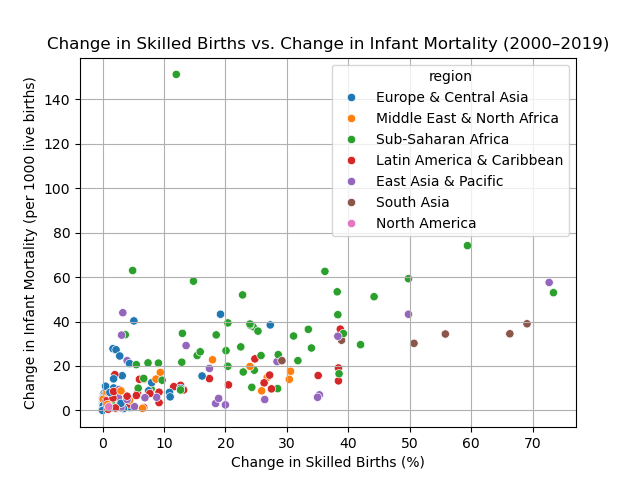
\includegraphics[keepaspectratio]{part3_images/change_skilled_births_vs_infant_mortality.png}}

}

\caption{Figure 7}

\end{figure}%

To explore the relationship between maternal healthcare access and
infant survival outcomes, we plotted the change in births attended by
skilled health staff against the change in infant mortality rates
between 2000 and 2019.

Each point in the scatterplot represents a region, color-coded.

We used the following metrics:

\begin{itemize}
\tightlist
\item
  X-axis: Change in the percentage of births attended by skilled health
  staff (\%)
\item
  Y-axis: Change in infant mortality (per 1,000 live births)
\end{itemize}

This visual helps assess whether increases in skilled birth attendance
are associated with better infant health outcomes, and whether this
trend is consistent across regions.

Many countries that experienced an increase in skilled birth attendance
from 2000 to 2019 also saw a decrease in infant mortality (or greater
change in infant mortality), especially in Sub-Saharan Africa, South
Asia, and East Asia \& Pacific. This suggests a negative correlation: as
more births are attended by skilled health staff, fewer infants die.

\begin{figure}[H]

{\centering \pandocbounded{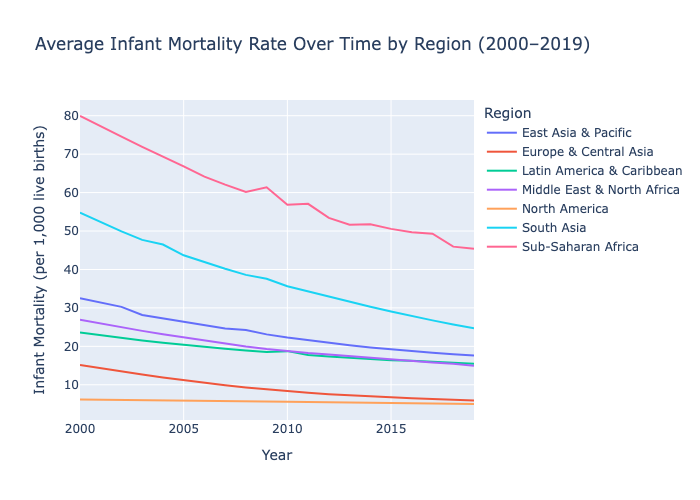
\includegraphics[keepaspectratio]{part3_images/average_infant_mortality_by_region.png}}

}

\caption{Figure 8}

\end{figure}%

To understand trends in infant survival across global regions, we
plotted average infant mortality rates from 2000 to 2019.

Each line represents a different world region, showing changes in infant
deaths per 1,000 live births over time.

Key insights from this visualization include:

\begin{itemize}
\tightlist
\item
  All regions experienced a decline in infant mortality rates over the
  20-year period.
\item
  Sub-Saharan Africa had the highest rates throughout, though it also
  saw significant improvement---from around 80 deaths per 1,000 live
  births in 2000 to below 50 by 2019.
\item
  South Asia also made significant progress closing the gap with regions
  that have lower infant mortality rates.
\item
  Regions like Europe \& Central Asia and North America maintained the
  lowest infant mortality rates, with steady improvements, though the
  overall changes were smaller.
\end{itemize}

These patterns reflect global progress in child health and survival,
while highlighting persistent disparities across regions. The overall
downward trend is consistent with increased access to healthcare and
maternal services observed during this time.

\begin{figure}[H]

{\centering \pandocbounded{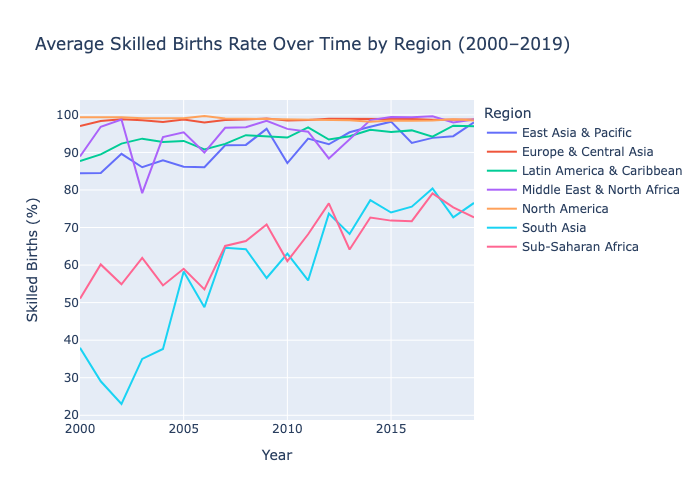
\includegraphics[keepaspectratio]{part3_images/average_skilled_births_by_region.png}}

}

\caption{Figure 9}

\end{figure}%

To track improvements in maternal healthcare access globally, we
visualized the average percentage of births attended by skilled health
staff across world regions from 2000 to 2019.

Each line represents a region, illustrating how skilled birth attendance
has evolved over time.

Key insights from the figure include:

\begin{itemize}
\tightlist
\item
  Regions like Europe \& Central Asia and North America consistently
  maintained near-universal skilled birth attendance, with rates close
  to 100\% .
\item
  East Asia \& Pacific, Latin America \& Caribbean, and Middle East \&
  North Africa also exhibited high and relatively stable skilled birth
  rates, typically above 90\%.
\item
  Sub-Saharan Africa and South Asia, which started with the lowest
  skilled birth attendance rates in 2000, showed substantial improvement
  over the two decades. South Asia, in particular, saw an increase from
  around 35\% to over 70\%.
\end{itemize}

The upward trends in these regions reflect significant investments in
maternal health services and broader healthcare access.

This visualization highlights regional disparities in maternal
healthcare but also showcases meaningful global progress, particularly
in regions with historically lower access to skilled care during
childbirth.

\section{Conclusion and Further
Reading}\label{conclusion-and-further-reading}

This project investigates the relationships between public health and
population dynamics using World Bank data to reveal patterns across
regions and income levels. Focusing on three indicator pairs, we analyze
how demographic and health factors interact, including adolescent
fertility rate and population growth, age dependency ratio and life
expectancy at birth, and births attended by skilled health staff and
infant mortality rates.

Both pairs 1 and 2 supported trends across countries of different income
groups, attributed to phenomena associated with demographic transition.
Low income countries have experienced the greatest decreases in
adolescent fertility rates but also the largest increase in population
growth rates. This highlights the fact that fertility rates in not
adolescents, but older population as well as a country's overall
improvements in areas such as access to food, healthcare, sanitation,
and economic development. Likewise, the more pronounced decreases in
dependency ratios lower-middle and upper-middle income countries as they
transition to highly developed economies reflect a shift in the
demographics working class to older groups, as well as also having a
more pronounced increase in life expectancy as opposed to highly
developed countries, where life expectancy is already approaching its
human limits. These indicators and their trajectories aren't necessarily
the sole cause of one another, but are intertwined with and influence
one another and change accordingly with a country's point along
demographic transition into highly developed economies.

For pair 3, the analysis shows that increased skilled birth attendance
is strongly associated with declines in infant mortality globally, with
significant progress in regions like Sub-Saharan Africa and South Asia
despite ongoing disparities. A systematic review of 41 African countries
demonstrated that a 10\% increase in skilled birth attendance
corresponded with a 6\% reduction in neonatal mortality, highlighting
the critical impact of skilled healthcare during childbirth on infant
survival (Berhan and Berhan 2014). Similarly, a national survey in
Lesotho found that births not attended by skilled health personnel had
twice the risk of neonatal death compared to those with skilled
attendants, directly supporting the finding that increased skilled birth
attendance is linked to lower infant mortality rates (Baruwa, Amoateng,
and Mkwananzi 2021).

\phantomsection\label{refs}
\begin{CSLReferences}{1}{0}
\bibitem[\citeproctext]{ref-baruwa2021association}
Baruwa, Ololade Julius, Acheampong Yaw Amoateng, and Sibusiso Mkwananzi.
2021. {``Association Between Type of Birth Attendants and Neonatal
Mortality: Evidence from a National Survey.''} \emph{African Health
Sciences} 21 (4): 1870--76.

\bibitem[\citeproctext]{ref-berhan2014skilled}
Berhan, Yifru, and Asres Berhan. 2014. {``Skilled Health Personnel
Attended Delivery as a Proxy Indicator for Maternal and Perinatal
Mortality: A Systematic Review.''} \emph{Ethiopian Journal of Health
Sciences} 24: 69--80.

\bibitem[\citeproctext]{ref-harwood2004current}
Harwood, Rowan H, Avan Aihie Sayer, and Miriam Hirschfeld. 2004.
{``Current and Future Worldwide Prevalence of Dependency, Its
Relationship to Total Population, and Dependency Ratios.''}
\emph{Bulletin of the World Health Organization} 82: 251--58.

\bibitem[\citeproctext]{ref-Murray2018}
Murray, Christopher J L, Charlton S K H Callender, Xie Rachel Kulikoff,
Vinay Srinivasan, Degu Abate, Kalkidan Hassen Abate, Solomon M Abay, et
al. 2018. {``Population and Fertility by Age and Sex for 195 Countries
and Territories, 1950--2017: A Systematic Analysis for the Global Burden
of Disease Study 2017.''} \emph{The Lancet} 392 (10159): 1995--2051.
\url{https://doi.org/10.1016/s0140-6736(18)32278-5}.

\bibitem[\citeproctext]{ref-pablos2015demographic}
Pablos-Mendez, Ariel, Scott R Radloff, Kamiar Khajavi, and Sally Ann
Dunst. 2015. {``The Demographic Stretch of the Arc of Life: Social and
Cultural Changes That Follow the Demographic Transition.''} \emph{Global
Health: Science and Practice} 3 (3): 341--51.

\end{CSLReferences}




\end{document}
